
\begin{figure}

\begin{center}

\fbox{
{\ttfamily
\begin{alg}{4.0in}
for ( int i = 1; i < n; i++ ) \{ \+\\
    double x = A[i]; toInsert.setWeight( A[i] ); \\
    toInsert.setX( xCoord[i] ); \\
    endStep(); \\
    int j = i - 1; \\
    while ( j >= 0 \&\& A[j] > x ) \{ \+\\  
        beginStep(); \\
        toInsert.setX( xCoord[j] ); \\
        nodes[j].setSelected( true ); \\
        endStep(); beginStep(); \\
        A[j+1] = A[j]; nodes[j+1].setWeight( A[j] ); \\
        nodes[j].unMark(); \\
        nodes[j].setSelected( false ); \\
        nodes[j+1].mark(); \\
        endStep(); \\
        j = j - 1; \-\\
    \} \\
    beginStep(); \\
    A[j+1] = x; nodes[j+1].setWeight( x ); \\
    nodes[j+1].mark(); \-\\
\}
\end{alg}
} % ttfamily
} % fbox

\bigskip

\fbox{
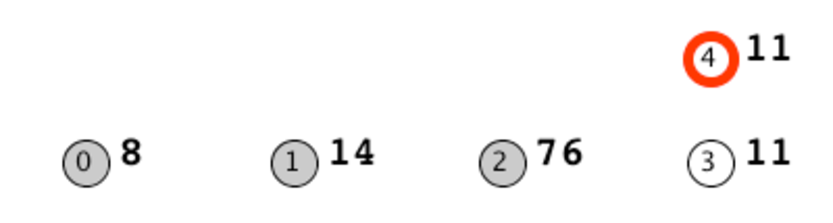
\includegraphics[scale=0.4]{X_is_1}
}

\smallskip
(a) Starting to insert \verb$x = A[3]$.

\bigskip
\fbox{
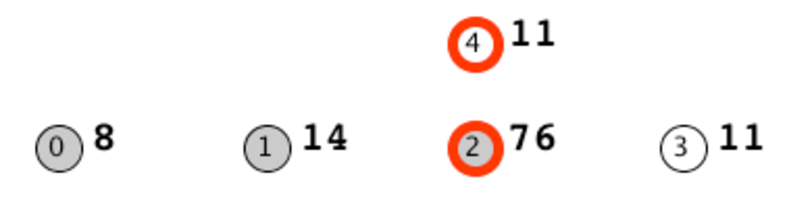
\includegraphics[scale=0.4]{X_is_2}
}

\smallskip
(b) Comparing \verb$x$ with \verb$A[2]$.

\bigskip
\fbox{
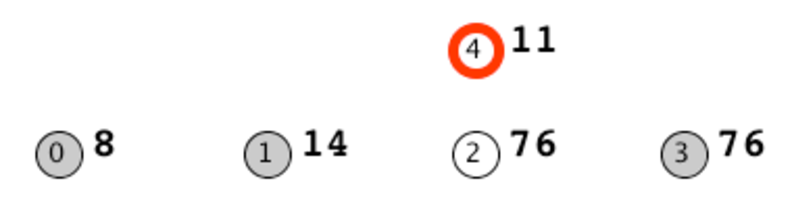
\includegraphics[scale=0.4]{X_is_3}
}

\smallskip
(c) \verb$A[2] > x$ so \verb$A[3] = A[2]$.

\end{center}

\caption{The insertion sort algorithm
and three steps in the animation.}
\label{fig:insertion_sort_animation}
\end{figure}
